\title{Naive Bayes}
\label{chp:naive-bayes}
\author{Leandro L. Minku}
\institute{School of Computer Science, University of Birmingham, UK}
\maketitle


The process of learning predictive models from data typically involves uncertainty. For instance, different models could potentially be created to describe the same data, and different predictions could be given to future data. The decision of which model to adopt and which prediction to make thus involves uncertainty \cite{ProbabilisticLearningNature}. This chapter will introduce you to probabilistic learning, which captures uncertainty through probability theory. In particular, we will cover a machine learning approach called Na\"ive Bayes. Despite being a relatively simple technique, Na\"ive Bayes often outperforms more complex approaches \cite{ElementsStatisticalLearning}, being a good place to start learning the topic of probabilistic learning.

This chapter assumes that you are relatively familiar with probability concepts such as random variables; probability distributions; probability mass functions; probability density functions; prior, marginal or unconditional probabilities; conditional or posterior probabilities; and joint probability distributions. If you are unfamiliar with these terms, we suggest you to read Section 13.2.1 and 13.2.2 of \cite{RussellNorvig} or Chapter 6 of \cite{MathsForML} for a deeper understanding of this chapter.

Section \ref{sec:bayes-theorem}  introduces the Bayes theorem upon which Na\"ive Bayes is based and the relationship that this theorem has with classification. Section \ref{sec:nb-categorical} introduces the Na\"ive Bayes approach for categorical input variables. Section \ref{sec:nb-numeric} introduces Na\"ive Bayes for numeric input variables.


\section{The Bayes Theorem and Its Relationship With Classification}
\label{sec:bayes-theorem}

Consider a machine learning problem with input variables $\mathbf{x}$ and output variable $y$, where $\mathbf{x} = (x_1,x_2,\cdots,x_d)$ is a $d$-dimensional vector, $\mathbf{x} \in \mathcal{X}$, $y \in \mathcal{Y}$, $\mathcal{X}$ is the input space and $\mathcal{Y}$ is the output space of the problem. In regression problems, $\mathcal{Y} = \mathbb{R}$, whereas in classification problems $\mathcal{Y}$ is a set of categories. In this chapter, we will focus on classification problems. 

In probabilistic learning, we consider that $(\mathbf{x},y)$ are random variables drawn from a fixed, albeit unknown joint probability distribution $p(\mathbf{x},y)$ \footnote{There are also machine learning problems where  $p(\mathbf{x},y)$ is not fixed. However, we will not cover them in this book. For more information on those problems, we recommend \cite{MLForDataStreams}.}. In particular, in supervised learning, we assume that a training set of examples is available, consisting of $N$ samples\footnote{In some machine learning problems, the training set may not be fully available beforehand. Instead, training examples may arrive over time.} drawn from $p(\mathbf{x},y)$:

\begin{equation} \mathcal{T} = \{(\mathbf{a}^{(1)},c^{(1)}),(\mathbf{a}^{(2)},c^{(2)}),\cdots, (\mathbf{a}^{(N)},c^{(N)})\}, \label{eq:training-set} \end{equation}

\noindent where $\mathbf{a}^{(i)},c^{(i)}$ represent the values of the input and output variables\footnote{In this chapter, we will use letters such as $\mathbf{a}^{(i)},c^{(i)}$ to represent the values of the input and output variables instead of using their corresponding indexed variable names $\mathbf{x}^{(i)},y^{(i)}$ in sample $i$. This will enable us to distinguish more explicitly between the variables and their values, which can be useful when discussing Na\"ive Bayes.}. 
Supervised learning in then considered to be the problem of using the training set $\mathcal{T}$ to learn a model $f: \mathcal{X} \rightarrow \mathcal{Y}$ able to generalise to unseen examples from $p(\mathbf{x},y)$. %In probabilistic learning, this model is a probabilistic model. 
%Learning occurs through the transformation of prior probability distributions (defined before observing data) into posterior probability distributions (after observing the training set) \cite{ProbabilisticLearningNature}.

Based on the product rule from probability theory, the joint probability distribution $p(\mathbf{x},y)$ can be written as:

\[ p(\mathbf{x},y) = p(y|\mathbf{x}) p(\mathbf{x}) = p(\mathbf{x}|y) p(y),\]

\noindent where $p(y|\mathbf{x})$ is the conditional distribution of $y$, $p(\mathbf{x})$ is the unconditional or marginal distribution of $\mathbf{x}$, $p(\mathbf{x}|y)$ is the conditional distribution of $\mathbf{x}$ and $p(y)$ is the prior probability of $y$. From this, we have that

\[p(y|\mathbf{x}) = \frac{p(y) p(\mathbf{x}|y)}{p(\mathbf{x})}.\]

Therefore, given an example with known value of $\mathbf{x}=\mathbf{a}$, one can calculate the probability of it belonging to a given class $y = c$ as

\begin{equation}p(y=c|\mathbf{x}=\mathbf{a}) = \frac{p(y=c) p(\mathbf{x}=\mathbf{a}|y=c)}{p(\mathbf{x}=\mathbf{a})}. \label{eq:bayes-theorem} \end{equation}

\noindent This is known as the Bayes Theorem. To simplify the writing, whenever it is not ambiguous, we will write this as

\[p(c|\mathbf{a}) = \frac{p(c) (\mathbf{a}|c)}{p(\mathbf{a})}.\]

Such probabilities can be used to make inferences, i.e., to predict the class $c$ given the observed input values $\mathbf{a}$. In particular, one can compute $p(c|\mathbf{a})$ for every possible class $c$, and predict the class associated to the highest probability $p(c|\mathbf{a})$. This means that these probabilities can work as our model $f: \mathcal{X} \rightarrow \mathcal{Y}$. 
But how to compute these probabilities?
For that, in supervised learning, we can rely on the fact that we have access to a training set $\mathcal{T}$. This training set can be used to create frequency tables that enable us to compute these probabilities. 

Let's have a look at a simplified problem to illustrate how this works. Consider a problem where we have a single input variable $x_1$ representing whether a person eats healthy foods and a output variable $y$ corresponding to whether that person is developing cancer. The problem is to predict whether the person is developing cancer based on whether they eat healthy foods. In this problem, we will refer to $x_1$ as ``healthy'' and $y$ as ``cancer'', to facilitate reading. 

Assume we have access to the training set corresponding to six people shown in Table \ref{tab:dataset-single-input}. We can compute the number of times that each different value of the input and output variables occur together as shown in the frequency table given in Table \ref{tab:frequency-single-input}. Then, let's say that we have received a new test instance corresponding to a person who does not eat healthy foods (i.e., $\text{healthy} = \textit{no}$) and wish to predict whether this person is developing cancer by applying the Bayes Theorem\footnote{We could potentially compute $p(\text{cancer}=\textit{yes}|\text{healthy} = \textit{no})$ and $p(\text{cancer}=\textit{no}|\text{healthy} = \textit{no})$ directly from the frequency tables without having to apply the Bayes Theorem. However, the intention of this example is to show that we can compute them by applying the Bayes Theorem, which will be useful to learn Na\"{i}ve Bayes in the next section.}. 

\begin{table}[ht]
\centering
\caption{An Illustrative Dataset With A Single Input Variable} \label{tab:dataset-single-input}
\begin{tabular}{|c|c|} \hline
$x_1$ (healthy) & $y$ (cancer) \\ \hline
\textit{no} & \textit{yes} \\
\textit{no} & \textit{yes} \\
\textit{yes} & \textit{yes} \\
\textit{yes} & \textit{no} \\
\textit{yes} & \textit{no} \\
\textit{no} & \textit{no} \\ \hline
\end{tabular}
\end{table}

\begin{table}[ht]
\centering
\caption{An Illustrative Frequency Table For The Single Input Variable Dataset From Table \ref{tab:dataset-single-input}} \label{tab:frequency-single-input}
\begin{tabular}{|l|c|c|c|} \hline
 & cancer = \textit{no} & cancer= \textit{yes} & total \\ \hline
healthy = \textit{no} & 1 & 2 & 3 \\ \hline
healthy = \textit{yes} & 2 & 1 & 3 \\ \hline
total & 3 & 3 & 6 \\ \hline
\end{tabular}
\end{table}

From Eq.~\ref{eq:bayes-theorem}, we have that

\[ p(\text{cancer}=\textit{yes}|\text{healthy} = \textit{no}) = 
\frac{p(\text{cancer}=\textit{yes}) p(\text{healthy} = \textit{no}|\text{cancer}=\textit{yes})}{p(\text{healthy} = \textit{no})} \]

and

\[p(\text{cancer}=\textit{no}|\text{healthy} = \textit{no}) =
\frac{p(\text{cancer}=\textit{no}) p(\text{healthy} = \textit{no}|\text{cancer}=\textit{no})}{p(\text{healthy} = \textit{no})} .\]

\vspace{1cm}
Based on the frequency table given in Table \ref{tab:frequency-single-input}, we have that

\begin{itemize}
\item $p(\text{cancer}=\textit{yes}) = 3/6$, as $3$ in $6$ people had cancer;
\item $p(\text{healthy} = \textit{no}|\text{cancer}=\textit{yes}) = 2/3$, as $2$ in $3$ of the people with cancer did not eat healthy foods;
\item $p(\text{cancer}=\textit{no}) = 3/6$, as $3$ in $6$ people did not have cancer;
\item $p(\text{healthy} = \textit{no}|\text{cancer}=\textit{no}) = 1/3$, as $1$ in $3$ of the people with cancer ate healthy foods;
\item $p(\text{healthy} = \textit{no}) = 3/6$, as $3$ in $6$ people did not eat healthy foods.
\end{itemize}

\vspace{1cm}
Therefore,

\[p(\text{cancer}=\textit{yes}|\text{healthy} = \textit{no}) = \frac{3/6 \times 2/3}{3/6} \approx 0.67.\]

\[p(\text{cancer}=\textit{no}|\text{healthy} = \textit{no}) = \frac{3/6 \times 1/3}{3/6} \approx 0.33.\]

As $p(\text{cancer}=\textit{yes}|\text{healthy} = \textit{no}) > p(\text{cancer}=\textit{no}|\text{healthy} = \textit{no})$, it would be reasonable to predict that the class is $\text{cancer} = \textit{yes}$.


It is worth noting that the denominator $p(\mathbf{a})$ of the Bayes Theorem ($p(\text{healthy} = \textit{no})$ in the example above) works as a normalisation factor to ensure that the probabilities of the test instance to belong to each different possible class sums to one, i.e.:

\[ \sum_{c \in \mathcal{Y}} p(c|\mathbf{a}) = 1\]


We could replace $p(\mathbf{a})$ by the factor $\beta$ shown below and achieve the same normalisation effect:

\[ \beta = \sum_{c \in \mathcal{Y}} p(c) p(\mathbf{a}|c) . \]

If we set $\alpha = 1 / \beta$, then the Bayes Theorem becomes:

\begin{equation}p(c|\mathbf{a}) = \alpha p(c) p(\mathbf{a}|c) . \label{eq:nb-alpha}\end{equation}

In the next section, it will be useful to explicitly use $\alpha$ instead of $p(\mathbf{a})$, as the assumptions made by Na\"{i}ve Bayes will cause $p(\mathbf{a})$ not to work as a normalising factor anymore, potentially resulting in probabilities that would not sum to 1, i.e., in values that are not really probabilities.

\section{Na\"{i}ve Bayes for Categorical Input Variables}
\label{sec:nb-categorical}

The Bayes Theorem can be written as follows for $d$ input variables:

\[p(c|\mathbf{a}) = \alpha p(c) p(\mathbf{a}|c)  = \alpha p(c) p(a_1,a_2,\cdots,a_d|c).\]

As the probability $p(a_1,a_2,\cdots,a_d|c)$ corresponds to the probability of a given combination of values $a_1,a_2,\cdots,a_d$ for the input variables being observed together given a class $c$, each row of our frequency table would correspond to a different combination of values for the input variables. For example, consider a problem with two input variables, where the first input variable $x_1$ represents whether the person eats healthy foods and the second input variable $x_2$ represents whether this person is suffering from pain. Assume that we would like to predict whether a person is developing cancer (output variable $y$) based on these input variables. For a problem with the dataset shown in Table \ref{tab:dataset-2dim}, we could have the frequency table shown in Table \ref{tab:frequency-2dim}. For problems with large numbers of input variables and many possible values for such variables, the number of rows in this kind of frequency table would quickly become intractable. 


\begin{table}[ht]
\centering
\caption{An Illustrative Dataset With Two Input Variables} \label{tab:dataset-2dim}
\begin{tabular}{|c|c|c|} \hline
$x_1$ (healthy) & $x_2$ (pain) & $y$ (cancer) \\ \hline
\textit{no} & \textit{yes} & \textit{yes} \\
\textit{no} & \textit{yes} & \textit{yes} \\
\textit{yes} & \textit{yes} & \textit{yes} \\
\textit{yes} & \textit{no} & \textit{no} \\
\textit{yes} & \textit{no} & \textit{no} \\
\textit{no} & \textit{no} & \textit{no} \\ \hline
\end{tabular}
\end{table}

\begin{table}[ht]
\centering
\caption{An Illustrative Frequency Table For The Two Input Variable Dataset From Table \ref{tab:dataset-2dim}} \label{tab:frequency-2dim}
\begin{tabular}{|l|c|c|c|} \hline
 & cancer = \textit{no}  & cancer= \textit{yes} & total \\ \hline
healthy = \textit{no} and pain = \textit{no} & 1 & 0 & 1 \\ \hline
healthy = \textit{no} and pain = \textit{yes} & 0 & 2 & 2 \\ \hline
healthy = \textit{yes} and pain = \textit{no} & 2 & 0 & 2 \\ \hline
healthy = \textit{yes} and pain = \textit{yes} & 0 & 1 & 1 \\ \hline
total & 3 & 3 & 6 \\ \hline
\end{tabular}
\end{table}


Na\"{i}ve Bayes is a machine learning approach that deals with this issue by making the assumption that the input variables are conditionally independent of each other given the output variable. A variable $x_1$ is conditionally independent of $x_2$ given the output variable $y$ if the following condition is satisfied:

\[ p(x_1|x_2,y) = p(x_1|y) . \]

\noindent This means that, if we know the value of $y$, we do not need to know the value of $x_2$ to determine the value of $x_1$. By making this assumption, we can say that:

\[ P(a_1,a_2,\cdots,a_d|c) = \prod_{i=1}^d p(a_i|c). \]

\noindent By replacing this in the Bayes Theorem (Equation \ref{eq:nb-alpha}), we get:

\begin{equation}p(c|\mathbf{a}) = \alpha p(c) \prod_{i=1}^d p(a_i|c),\label{eq:naive-bayes}
\end{equation}

\noindent where 

\[\alpha = \frac{1}{\sum_{c \in \mathcal{Y}} \left( p(c) \prod_{i=1}^d p(a_i|c)\right)} .\]

Na\"{i}ve Bayes uses Eq.~\ref{eq:naive-bayes} to calculate $p(c|\mathbf{a})$ in order to predict the class associated to a given example whose input variables have value $\mathbf{a}$. This means that a separate frequency table can be created for each input variable, leading to a total number of rows that grows linearly with the number of values that the input variables can assume. 

For example, let's consider again our problem of predicting whether a person is developing cancer based on whether they eat healthy foods and are experiencing pain. The training set for this problem is shown in Table \ref{tab:dataset-2dim}. The frequency tables corresponding to this training set would be the ones shown in Table \ref{tab:nb-frequency-2dim}.

\begin{table}[ht]
\centering
\caption{An Illustrative Frequency Table For The Two Input Variable Dataset From Table \ref{tab:dataset-2dim}} \label{tab:nb-frequency-2dim}
\begin{subtable}[h]{0.49\textwidth}
\caption{Frequency Table For $x_1$ (Healthy)}
\begin{tabular}{|l|c|c|c|} \hline
 & cancer = \textit{no} & cancer= \textit{yes} & total \\ \hline
healthy = \textit{no} & 1 & 2 & 3 \\ \hline
healthy = \textit{yes} & 2 & 1 & 3 \\ \hline
total & 3 & 3 & 6 \\ \hline
\end{tabular}
\end{subtable}
\vspace{0.5cm}

\begin{subtable}[h]{0.49\textwidth}
\caption{Frequency Table For $x_2$ (Pain)}
\begin{tabular}{|l|c|c|c|} \hline
 & cancer = \textit{no} & cancer= \textit{yes} & total \\ \hline
pain = \textit{no} & 3 & 0 & 3 \\ \hline
pain = \textit{yes} & 0 & 3 & 3 \\ \hline
total & 3 & 3 & 6 \\ \hline
\end{tabular}
\end{subtable}
\end{table}

Let's assume that we wish to predict whether a person who eats healthy foods ($\text{healthy} = \textit{yes}$) and is experiencing pain ($\text{pain} = \textit{yes}$) is developing cancer. We would need to compute the following:

\[p(\text{cancer} = \textit{yes}| \text{healthy} = \textit{yes}, \text{pain} = \textit{yes}) = \]
\[\alpha p(\text{cancer} = \textit{yes}) \times p(\text{healthy} = \textit{yes} | \text{cancer} = \textit{yes}) \times p(\text{pain} = \textit{yes} | \text{cancer} = \textit{yes}) = \]
\[ \alpha \times 3/6 \times 1/3 \times 3/3 = \alpha \times 1/6\]

\vspace{0.5cm}
\[p(\text{cancer} = \textit{no}| \text{healthy} = \textit{yes}, \text{pain} = \textit{yes}) = \]
\[\alpha p(\text{cancer} = \textit{no}) \times p(\text{healthy} = \textit{yes} | \text{cancer} = \textit{no}) \times p(\text{pain} = \textit{yes} | \text{cancer} = \textit{no}) = \]
\[ \alpha \times 3/6 \times 2/3 \times 0/3 = 0\]

\noindent where 

\[\alpha = \frac{1}{3/6 \times 1/3 \times 3/3 + 3/6 \times 2/3 \times 0/3} = 6. \]

\vspace{0.5cm}
As $p(\text{cancer} = \textit{yes}| \text{healthy} = \textit{yes}, \text{pain} = \textit{yes})  > p(\text{cancer} = \textit{no}| \text{healthy} = \textit{yes}, \text{pain} = \textit{yes})$, Na\"{i}ve Bayes predicts that the person is developing cancer.

Note that in the calculations above, the whole probability of the person not developing cancer became zero, because $p(\text{pain} = \textit{yes} | \text{cancer} = \textit{no}) = 0$. In fact, even if there had been many other input variables in this problem, all with values suggesting that this person was not developing cancer, the whole probability of the person not developing cancer would still become zero, just because $p(\text{pain} = yes | \text{cancer} = \textit{no}) = 0$. This would lead to several inaccuracies on Na\"{i}ve Bayes' predictions. 

One way to avoid this problem is to adopt Laplace Smoothing. This consists in summing a small value $\epsilon > 0$ to every frequency value in the frequency table, and adjusting the total cells accordingly. And example for $\epsilon = 1$  is shown in Table \ref{tab:nb-laplace-frequency-2dim}.

\begin{table}[ht]
\centering
\caption{An Illustrative Frequency Table With Laplace Smoothing For The Two Input Variable Dataset From Table \ref{tab:dataset-2dim}} \label{tab:nb-laplace-frequency-2dim}
\begin{subtable}[h]{0.49\textwidth}
\caption{Frequency Table For $x_1$ (Healthy)} \label{tab:nb-laplace-frequency-2dim-healthy}
\begin{tabular}{|l|c|c|c|} \hline
 & cancer = \textit{no} & cancer= \textit{yes} & total \\ \hline
healthy = \textit{no} & 1+1=2 & 2+1=3 & 5 \\ \hline
healthy = \textit{yes} & 2+1=3 & 1+1=2 & 5 \\ \hline
total & 5 & 5 & 10 \\ \hline
\end{tabular}
\end{subtable}
\vspace{0.5cm}

\begin{subtable}[h]{0.49\textwidth}
\caption{Frequency Table For $x_2$ (Pain)}
\begin{tabular}{|l|c|c|c|} \hline
 & cancer = \textit{no} & cancer= \textit{yes} & total \\ \hline
pain = \textit{no} & 3+1=4 & 0+1=1 & 5 \\ \hline
pain = \textit{yes} & 0+1=1 & 3+1=4 & 5 \\ \hline
total & 5 & 5 & 10 \\ \hline
\end{tabular}
\end{subtable}
\end{table}

When computing the probabilities for Eq.~\ref{eq:naive-bayes}, the values of $p(a_i|c)$ should be computed based on the updated tables, whereas $p(c)$ is still calculated based on the original tables (without Laplace Smoothing) \footnote{Try out Exercise \ref{ex:laplace} to understand why.}.  For instance, the calculations to predict whether a person who eats healthy foods and is experiencing pain would be as follows:

\[p(\text{cancer} = \textit{yes}| \text{healthy} = \textit{yes}, \text{pain} = \textit{yes}) = \]
\[\alpha p(\text{cancer} = \textit{yes}) \times p(\text{healthy} = yes | \text{cancer} = \textit{yes}) \times p(\text{pain} = yes | \text{cancer} = \textit{yes}) = \]
\[ \alpha \times 3/6 \times 2/5 \times 4/5 = \alpha \times 8/50\]

\vspace{0.5cm}
\[p(\text{cancer} = \textit{no}| \text{healthy} = \textit{yes}, \text{pain} = \textit{yes}) = \]
\[\alpha p(\text{cancer} = \textit{no}) \times p(\text{healthy} = \textit{yes} | \text{cancer} = \textit{no}) \times p(\text{pain} = \textit{yes} | \text{cancer} = \textit{no}) = \]
\[ \alpha \times 3/6 \times 3/5 \times 1/5 = 3/50\]

\noindent where 

\[\alpha = \frac{1}{3/6 \times 2/5 \times 4/5 + 3/6 \times 3/5 \times 1/5} = 50/11 .\]

\vspace{0.5cm}
As $p(\text{cancer} = \textit{yes}| \text{healthy} = \textit{yes}, \text{pain} = \textit{yes})  > p(\text{cancer} = \textit{no}| \text{healthy} = \textit{yes}, \text{pain} = \textit{yes})$, Na\"{i}ve Bayes still predicts that the person is developing cancer in this example. However, in other examples the predicted class could potentially change when adopting Laplace Smoothing.

\section{Na\"{i}ve Bayes for Numeric Input Variables}
\label{sec:nb-numeric}

The Na\"{i}ve Bayes frequency tables explained in the previous section contain one row for each possible value of the input variables. When dealing with numeric input variables, it is infeasible to have one row for each possible numeric value. How can Na\"{i}ve Bayes deal with numeric input variables?

To gain some insight into that, it is worth observing that, when we are collecting frequency values for the frequency tables and transforming them into probabilities, we are actually learning probability mass functions. These are functions that give the probability of observing each possible value of a discrete random variable \cite{RussellNorvig,MathsForML}, e.g., of a categorical value in our machine learning problems. For instance, the figure below shows an example of probability mass function for $p(\text{healthy}|\text{cancer} = \textit{yes})$, obtained through the frequency table given in Table \ref{tab:nb-laplace-frequency-2dim-healthy}.

\begin{figure}[h]
\centering
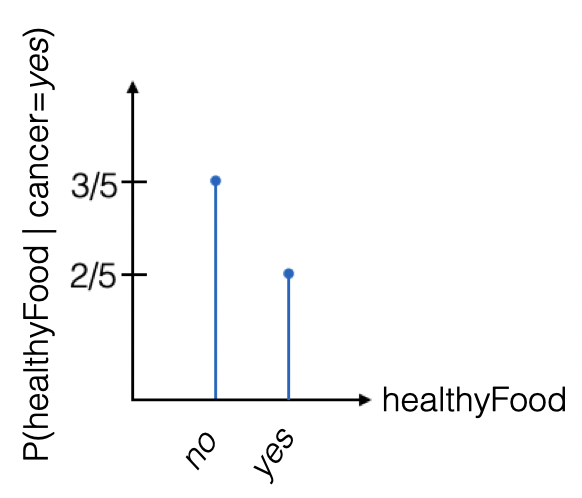
\includegraphics[scale=0.4]{"figures/nb-mass-function.png"} %"Part 3 - Learning Systems/Supervised Learning/Naive Bayes/
\caption{Probability Mass Function Obtained Through The Frequency Table Given in Table \ref{tab:nb-laplace-frequency-2dim-healthy}}
\end{figure}

For numeric input variables, we can learn probability density functions, instead of probability mass functions. Probability density functions represent the relative likelihood of observing different values of a given continuous random variable. Different from probability mass functions, the values of the relative likelihoods do not sum to one. Instead, the area under the curve formed by the function is equal to one \cite{MathsForML}. 

To be able to adopt probability density functions in Na\"{i}ve Bayes, one must choose what kind of probability density function to adopt. In most cases, a univariate Gaussian probability density function is used for each numeric input variable. This function can be written as follows for a given numeric input variable $x_i$:

\[ p(x_i|\mu,\sigma^2) = \frac{1}{\sqrt{2 \sigma^2 \pi}} e^{\frac{-(x_i - \mu)^2}{2 \sigma^2}}\]

\noindent where $\mu$ is a parameter corresponding to the mean of the distribution, $\sigma^2$ is a parameter corresponding to its variance, $\pi \approx 3.14159$ and $e \approx 2.71828$.

Learning then corresponds to setting appropriate values for the parameters $\mu$ and $\sigma^2$. In classification problems, every numeric input variable $x_i$ needs to be associated to a probability density function $p(x_i|c)$ for each of the possible values $c \in \mathcal{Y}$. In order to learn the parameters of these probability density functions, the training examples can be used. In particular, for a Gaussian probability density function associated to the input variable $x_i$ and the class value $c$, the mean $\mu$ is set as the mean of the $x$ values values of all training examples whose class value is $c$. The variance $\sigma^2$ is set as the variance of these values. Considering the training set defined in Eq.~\ref{eq:training-set} with $N$ training examples, the mean and variance of a variable $x_i$ is calculated as follows, respectively:

\[ \mu = \frac{1}{N} \sum_{(a^{(j)},c^{(j)}) \in \mathcal{T} \ \text{and} \ c^{(j)} = c} a_i^{(j)}, \]

and

\[ \sigma^2 = \frac{1}{N - 1} \sum_{(a^{(j)},c^{(j)}) \in \mathcal{T} \ \text{and} \ c^{(j)} = c} (a_i^{(j)} - \mu(x_i))^2 .\]

Let's have a look at an example of how to calculate this. Assume that we need to predict whether a person is developing cancer (output variable $y$) based on whether they eat healthy foods (categorical input variable $x_1$) and on the amount of alcohol in units that they consume per month (numeric input variable $x_2$). The training set is shown in Table \ref{tab:dataset-2dim-numeric}.

\begin{table}[ht]
\centering
\caption{An Illustrative Dataset With A Categorical and A Numeric Input Variable} \label{tab:dataset-2dim-numeric}
\begin{tabular}{|c|c|c|} \hline
$x_1$ (healthy) & $x_2$ (alcohol) & $y$ (cancer) \\ \hline
\textit{no} & 40 & \textit{yes} \\
\textit{no} & 35 &  \textit{yes} \\
\textit{yes} & 60 &  \textit{yes} \\
\textit{yes} & 20 &  \textit{no} \\
\textit{yes} & 30 &  \textit{no} \\
\textit{no} & 17 &  \textit{no} \\ \hline
\end{tabular}
\end{table}

Consider that we decide to use Gaussian probability density functions for the numeric input variable alcohol ($x_2$). As this is a binary classification problem (where $\mathcal{Y} = \{\textit{yes},\textit{no}\}$ is a set of size 2), this means that we need to learn two Gaussian conditional probability density functions for alcohol: one for $\text{cancer}=\textit{yes}$ and one for $\text{cancer}=\textit{no}$.

For $\text{cancer} = \textit{yes}$, we calculate the mean and variance of the alcohol values of all training examples where $\text{cancer} = \textit{yes}$:

\[ \mu = \frac{40 + 35 + 60}{3} = 45,\]

\[ \sigma^2 = \frac{1}{3-1} [(40 - 45)^2+(35 - 45)^2+(60 - 45)^2] = 175.\]

For $\text{cancer} = \textit{no}$, we calculate the mean and variance of the alcohol values of all training examples where $\text{cancer} = \textit{no}$:

\[ \mu = \frac{20 + 30 + 17}{3} \approx 22.33,\]

\[ \sigma^2 = \frac{1}{3-1} [(20 - 22.33)^2+(30 - 22.33)^2+(17 - 22.33)^2] \approx 46.34.\]

Therefore, one of the Gaussian conditional probability density functions is $p(\text{alcohol}|\mu=45,\sigma^2=175)$ and the other is $p(\text{alcohol}|\mu=22.33,\sigma^2=46.34)$. Note that we are omitting $\text{cancer}=\textit{yes}$ and $\text{cancer}=\textit{no}$ when we write $p(\text{alcohol}|\mu=45,\sigma^2=175)$ and $p(\text{alcohol}|\mu=22.33,\sigma^2=46.34)$ because the $\mu$ and $\sigma^2$ values already capture $\text{cancer}=\textit{yes}$ and $\text{cancer}=\textit{no}$. However, we could also write $\text{cancer}=\textit{yes}$ and $\text{cancer}=\textit{no}$ explicitly if we wanted. These two functions are plotted in Figure \ref{fig:nb-gaussian-pdfs}.

\begin{figure}[h]
\centering
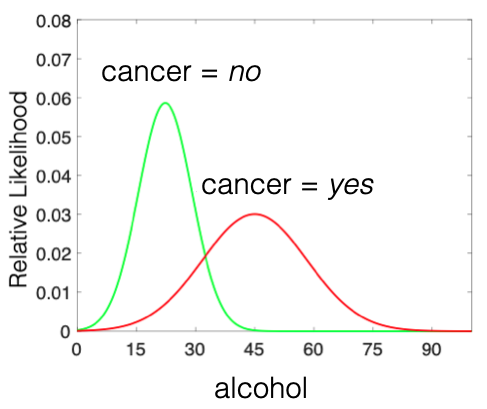
\includegraphics[scale=0.3]{"figures/nb-gaussian-pdfs.png"} %"Part 3 - Learning Systems/Supervised Learning/Naive Bayes/
\caption{Conditional Probability Density Functions For The Alcohol Variable Illustrative Dataset From Table \ref{tab:dataset-2dim-numeric}. $P(\text{alcohol}|\text{cancer}=\textit{no})$ is shown in green and $P(\text{alcohol}|\text{cancer}=\textit{yes})$ is shown in red.} \label{fig:nb-gaussian-pdfs}
\end{figure}


Once the parameters of the probability density functions are set, the values of $p(a_i|c)$ used in Equation \ref{eq:naive-bayes} can be taken from these functions. It is worth noting, though, that these values are relative likelihood instead of probabilities. However, the resulting $p(c|a_i)$ will still be probabilities due to the use of the normalising factor $\alpha$.

An example of prediction for this problem would be as follows. Consider that we wish to predict whether a person who does not eat healthy foods ($\text{healthy} = \textit{no}$) and consumes 20 units of alcohol per month ($\text{alcohol} = 20$) is developing cancer. The frequency tables for $x_1$ (healthy) with Laplace smoothing, the total number of training examples for $\text{cancer} = \textit{yes}$ and $\text{cancer} = \textit{no}$ and the parameters of the conditional probability density functions for $x_2$ (alcohol) computed based on the training set are shown in Tables \ref{tab:nb-laplace-frequency-2dim-healthy}, \ref{tab:num-examples-each-class} and \ref{tab:gaussian-parameters}, respectively.

\begin{table}[h]
\caption{Number of Training Examples From Each Class In The Training Set From Table \ref{tab:dataset-2dim-numeric}} \label{tab:num-examples-each-class}
\centering
\begin{tabular}{|c|c|c|}\hline
cancer = \textit{no} & cancer = \textit{yes} & total \\ \hline
3 & 3 & 6 \\ \hline
\end{tabular}
\end{table}


\begin{table}[h]
\caption{Parameters Of The Gaussian Conditional Probability Density Functions For The Training Set From Table \ref{tab:dataset-2dim-numeric}} \label{tab:gaussian-parameters}
\centering
\begin{tabular}{|c|c|c|}\hline
& cancer = \textit{no} & cancer= \textit{yes}  \\ \hline
$\mu$ & 22.33 & 45 \\ \hline
$\sigma^2$ & 46.34 & 175 \\ \hline
\end{tabular}
\end{table}

The probabilities $p(\text{cancer} = \textit{yes} | \text{healthy} = \textit{no}, \text{alcohol} = 20)$ and $p(\text{cancer} = \textit{no} | \text{healthy} = \textit{no}, \text{alcohol} = 20)$ are shown below:

\[ p(\text{cancer} = \textit{yes} | \text{healthy} = \textit{no}, \text{alcohol} = 20) = \]
\[ \alpha p(\text{cancer} = \textit{yes}) p(\text{healthy} = \textit{no} | \text{cancer} = \textit{yes}) p(\text{alcohol} = 20 | \text{cancer} = \textit{yes}) = \]
\[ \alpha \times 3/6 \times 3/5 \times 0.0051 = \alpha \times 0.00153 = 12.15\%\]

\vspace{0.5cm}
\[ p(\text{cancer} = \textit{no} | \text{healthy} = \textit{no}, \text{alcohol} = 20) = \]
\[ \alpha p(\text{cancer} = \textit{no}) p(\text{healthy} = \textit{no} | \text{cancer} = \textit{no}) p(\text{alcohol} = 20 | \text{cancer} = \textit{no}) = \]
\[ \alpha \times 3/6 \times 2/5 \times 0.0553 = \alpha \times 0.01106 = 87.85\%\]

\vspace{0.5cm}
\noindent where $\alpha = 1 / (0.00153 + 0.01106) \approx 79.43$.

\section{Strengths, Weaknesses and Applications of Na\"{i}ve Bayes}

Na\"{i}ve Bayes has several strengths and has been successfully applied in many different domains. Strengths include:
\begin{itemize}
\item Training is fast, as it requires only one pass through the data.
\item The relative probabilities computed by Na\"{i}ve Bayes have achieved good results for making predictions for many applications, such as text categorisation (e.g., spam detection \cite{Spam}), medical diagnosis \cite{MedicalDiagnosis}, software defect prediction \cite{SDP}, among others.
\end{itemize}

\noindent Na\"{i}ve Bayes' weaknesses include:
\begin{itemize}
\item It assumes conditional independence, which may be violated in many real world problems. 
\item Requires the choice of a probability density function for numeric input variables, which may not correspond to the true probability density function underlying the data.
\item Despite being frequently good for prediction purposes, the probability values themselves outputted by Na\"ive Bayes may not be good estimates of the actual probabilities.
%\item It does not work very well for regression problems, despite variations of it being available for this type of problems.
\end{itemize}

\section{Summary}

Na\"ive Bayes is a simple probabilistic learning approach that has demonstrated success in many applications. Its learning process involves creating frequency tables that correspond to probability mass functions for categorical input variables given the values of the output variable, or parameters of probability density functions corresponding to numeric input variables given the values of the output variable. Laplace smoothing is typically adopted to avoid misclassifications resulting from frequencies of zero associated to certain input and output values in the training set. Based on these functions, on the Bayes Theorem and on the conditional independence assumption, Na\"ive Bayes can then compute the probabilities of examples to belong to each given class, given the observed values of their input variables. These probabilities can then be used to decide which class to predict for these examples.


\section{Exercises}


\begin{enumerate}

\item \label{ex:frequency-tables} Consider the illustrative training set below, which was inspired by the real Heart Disease dataset from the UCI Machine Learning Repository\footnote{\url{https://archive.ics.uci.edu/ml/datasets/heart+disease}}.

\begin{center}
\begin{tabular}{|c|c|c|c|}\hline
$x_1$ (gender) & $x_2$ (smoker) & $x_3$ (paintype) & $y$ (heartdisease) \\ \hline
$female$ & $smokes$ & $angina$ & $yes$ \\ \hline
$male$ & $smokes$ & $angina$ & $yes$ \\ \hline
$male$ & $doesnt$ & $angina$ & $no$ \\ \hline
$male$ & $smokes$ & $nonangina$ & $no$ \\ \hline
$male$ & $doesnt$ & $nopain$ & $no$ \\ \hline
$female$ & $doesnt$ & $nopain$ & $no$ \\ \hline
$female$ & $doesnt$ & $angina$ & $yes$\\ \hline
\end{tabular} 
\end{center}

Create the frequency tables that compose the Na\"ive Bayes classifier for this training set using Laplace Smoothing with $\epsilon=1$. 

\item \label{ex:prediction} Determine the prediction that Na\"ive Bayes would give to the instance ($\text{gender}=female$, $\text{smoker}=smokes$, $\text{paintype}=nonangina$, heartdisease=?) using Laplace Smoothing with $\epsilon=1$, given the training set from Exercise \ref{ex:frequency-tables}.

\item \label{ex:laplace} Compute the probability $p(\text{heartdisease}=yes)$ based on the three different smoothed frequency tables that you have obtained in Exercise \ref{ex:prediction}, rather than based on the original frequency values of each class. Reflect about the results.

\end{enumerate}



\section{Exercise Answers}



\begin{enumerate}

\item \


\begin{tabular}{|c|c|c|c|}\hline
& heartdisease=$yes$ & heartdisease=$no$ & total \\ \hline
gender=$female$ & 3 & 2 & 5 \\ \hline
gender=$male$ & 2 & 4 & 6 \\ \hline
total & 5 & 6 & 11 \\ \hline
\end{tabular}

\vspace{0.5cm}

\begin{tabular}{|c|c|c|c|}\hline
& heartdisease=$yes$ & heartdisease=$no$ & total \\ \hline
smoker=$smokes$ & 3 & 2 & 5 \\ \hline
smoker=$doesnt$ & 2 & 4 & 6 \\ \hline
total & 5 & 6 & 11 \\ \hline
\end{tabular}

\vspace{0.5cm}

\begin{tabular}{|c|c|c|c|}\hline
& heartdisease=$yes$ & heartdisease=$no$ & total \\ \hline
paintype=$angina$& 4 & 2 & 6 \\ \hline
paintype=$nonangina$& 1 & 2 & 3 \\ \hline
paintype=$nopain$ & 1 & 3 & 4 \\ \hline
total & 6 & 7 & 13 \\ \hline
\end{tabular}

\vspace{0.5cm}

\item  In order to predict whether the person does or does not have disease, we need to compute $p(yes|female,smokes,nonangina)$ and $p(no|female,$ $smokes,nonangina)$. Then, we give a prediction corresponding to the higher probability.

For compute these probabilities, we need to instanciate Eq.~\ref{eq:naive-bayes}:

\[p(yes|female,smokes,nonangina) =\]
\[= \alpha P(yes) P(female|yes) P(smokes|yes) P(nonangina|yes)\]
\[= \alpha * 3/7 * 3/5 * 3/5 * 1/6\]
\[\approx \alpha * 0.0257 = 1 / (0.0257 + 0.01814) * 0.0257 \approx 0.59\]

\[P(no|female,smokes,nonangina) =\]
\[= \alpha * P(no) P(female|no) P(smokes|no) P(nonangina|no)\]
\[= \alpha * 4/7 * 2/6 * 2/6 * 2/7\]
\[\approx \alpha * 0.01814 = 1 / (0.0257 + 0.01814) * 0.01814 \approx 0.41\]

The $p(a|c)$ probabilities above are computed based on the frequency values from Exercise \ref{ex:frequency-tables}’s answer. For example, $P(female|yes) = 3/5$ because, according to the first column of the first table, 3 in 5 people who had disease were female. The probabilities $p(c)$ are still calculated based on the original frequencies (without Laplace smoothing).

As $p(yes|female,smokes,nonangina) > p(no|female,smokes,nonangina)$, Na\"ive Bayes would predict \textit{yes}, the person has the disease. However, as $p(yes|female,smokes,nonangina)$ is very close to $p(no|female,smokes,$ $nonangina)$, we can consider that Na\"ve Bayes is not very certain on the class being \textit{yes}.

\item We have three input variables. Two of them (gender and smoker) can assume two possible values ($female$/$male$ and $smokers$/$doesnt$). However, the other input variable (paintype) can assume three possible values ($angina$/$nonangina$/$nopain$). If we compute $p(\text{heartdisease}=yes)$ based on the first two smoothed tables, we get the value of $5/11 \approx 0.4545$. However, if we compute $p(\textit{heartdisease}=yes)$ based on the third smoothed table, we get the value $6/13 \approx 0.4615$. As we can see, these values are not the same, hindering the calculation of $p(yes)$.

\end{enumerate}


%Bishop’s book “Machine Learning and Pattern Recognition”, pages 45-46 (Combining Models).

%\vspace{.5cm}
%\noindent Russell and Norvig’s “Artificial Intelligence: A Modern Approach”, Sections 13.2 (Basic Probability Notation) to 13.6(The Wumpus World Revisited).


\bibliographystyle{unsrt}
\bibliography{bibliography}
